\section{Input signal design}
In this section, some commonly used perturbation signals will be discussed. An overview is given at the end of this section.
\subsection{White noise}
A continues white noise input ${u(t)}$ is characterized by the following properties;
	\begin{align}
			\mu_u &= E\{{u}(t)\} = 0  \\
			R_{uu} &= E\{{u}(t_1){u}(t_2)\} = \tfrac{1}{2}N\delta(t_1-t_2)
	\end{align}
Which basically means that the input $\mathbf{u}$ has zero mean ($\mu_u$) and each of the input indices are uncorrelated ($R_{uu}$) with each other. $N$ represents the number of samples and is infinite in a continues signal. Notice that the fourier transformation of a delta dirac function $\delta(t_1-t_2)$ gives simply one, the expected autospectral density of the white noise signal thus simply becomes;
	\begin{align}
			E\{S_{uu}\} = \tfrac{1}{2}N
	\end{align}
This is a very nice but strange property. It is nice because the average spectral density stays constant for all frequencies, allowing for infinite bandwidth identification. It also is a strange property, because this signal appears to have infinite power. However in practice we use discrete signals, which results in a finite bandwidth and thus finite power. In addition, we also may choose to apply a low pass filter to limit the frequency content to a certain range of interest.
		White noise is a random process, which makes it is impossible to predict future values. This is a nice property when identifying the human controller, since humans are capable of adapting their control strategy. Using random variables thus eliminates the possibility of using feedforward control. This assumption can be checked afterwards by analyzing the input ($y$) and output ($y$) covariance $C_{yu}$ as a function of the time difference $\tau$ between the two signals. 
	\begin{align}
			C_{yu} (\tau) = 0 \ \ , \ \tau < 0  
	\end{align}
This means that the output only depends on previous inputs, i.e. there exists a causal relationship between input (cause) and output (causality).
\subsection{Sine sweep}
The sine sweep is often used for structual vibration analsyis. Here the model subject to identification, is excited using a sine sweep, which most of the time starts at at low frequency and gradually builds up to higher frequencies. A typical definition of the swept sine is given by;
	\begin{align}
			u(t) = 2A\sin\left(\left[\pi(f_\textrm{max}-f_\textrm{min})\frac{t}{T} + 2\pi f_\textrm{min}\right] t\right)
	\end{align}
The autospectral density of this signal is constant between $f_\textrm{min}$ and $f_\textrm{max}$ and gradually decreases at $f>f_\textrm{max}$.
		Unfortuneatly the swept sine is a highly predictive signal, allowing a human controller to make use of feed forward control.
\subsection{Random phase multisine}
Finally we introduce the random phase multisine. Here we start by constructing the signal in the frequency domain and then convert the signal back to the time domain using a inverse Fourier transformation. The random multisine can be defined as follows:
	\begin{align}
			|U(\omega)| &= \begin{cases} 1 & \mathrm{for}  \ \omega_\textrm{min} \le \omega \le \omega_\textrm{max}, \\ 0 & \mathrm{for}\ \omega > \omega_\textrm{max} \end{cases}  \\
			\angle U(\omega) &= \begin{cases} \theta & \mathrm{for}  \ \omega_\textrm{min} \le \omega \le \omega_\textrm{max}, \\ 0 & \mathrm{for}\ \omega > \omega_\textrm{max} \end{cases}  
	\end{align}
Where $\theta$ is randomly distributed for each frequency $\omega$ according to an uniform probability density function.
Setting up signals in the frequency domain allows for easy autospectral density shaping. This is a nice feature, because we are generally interested in the frequency content of the input signal. Using this method allows the user to select one or multiple desired frequency bands. Unfortuneatly this kind of signal modelling in the frequency domain may result in unwanted peaks in the time domain.
\subsection{Crested multisine}
To reduce peak amplitudes while mainting the desired average power density, the phase can be optimized to fullfill these properties. The crest factor forms a usefull definition when optimizing the signal;
\begin{align}
    C = \frac{u_\textrm{max}}{u_\textrm{rms}} = \frac{\max(\mathbf{u})}{\sqrt{N^{-1}\mathbf{u}^T\mathbf{u}}}
\end{align}
The objective function will be to reduce the crest factor, the parameters subject to optimization will be the phase indices. It is beyond the scope of this report to explain the optimization algorithm in detail. What is important is that the resulting signal indeed has a significant lower crest factor. 
\subsection{Comparison}
A short overview of the various input signals is given in table.
		\begin{figure}
			\centering
				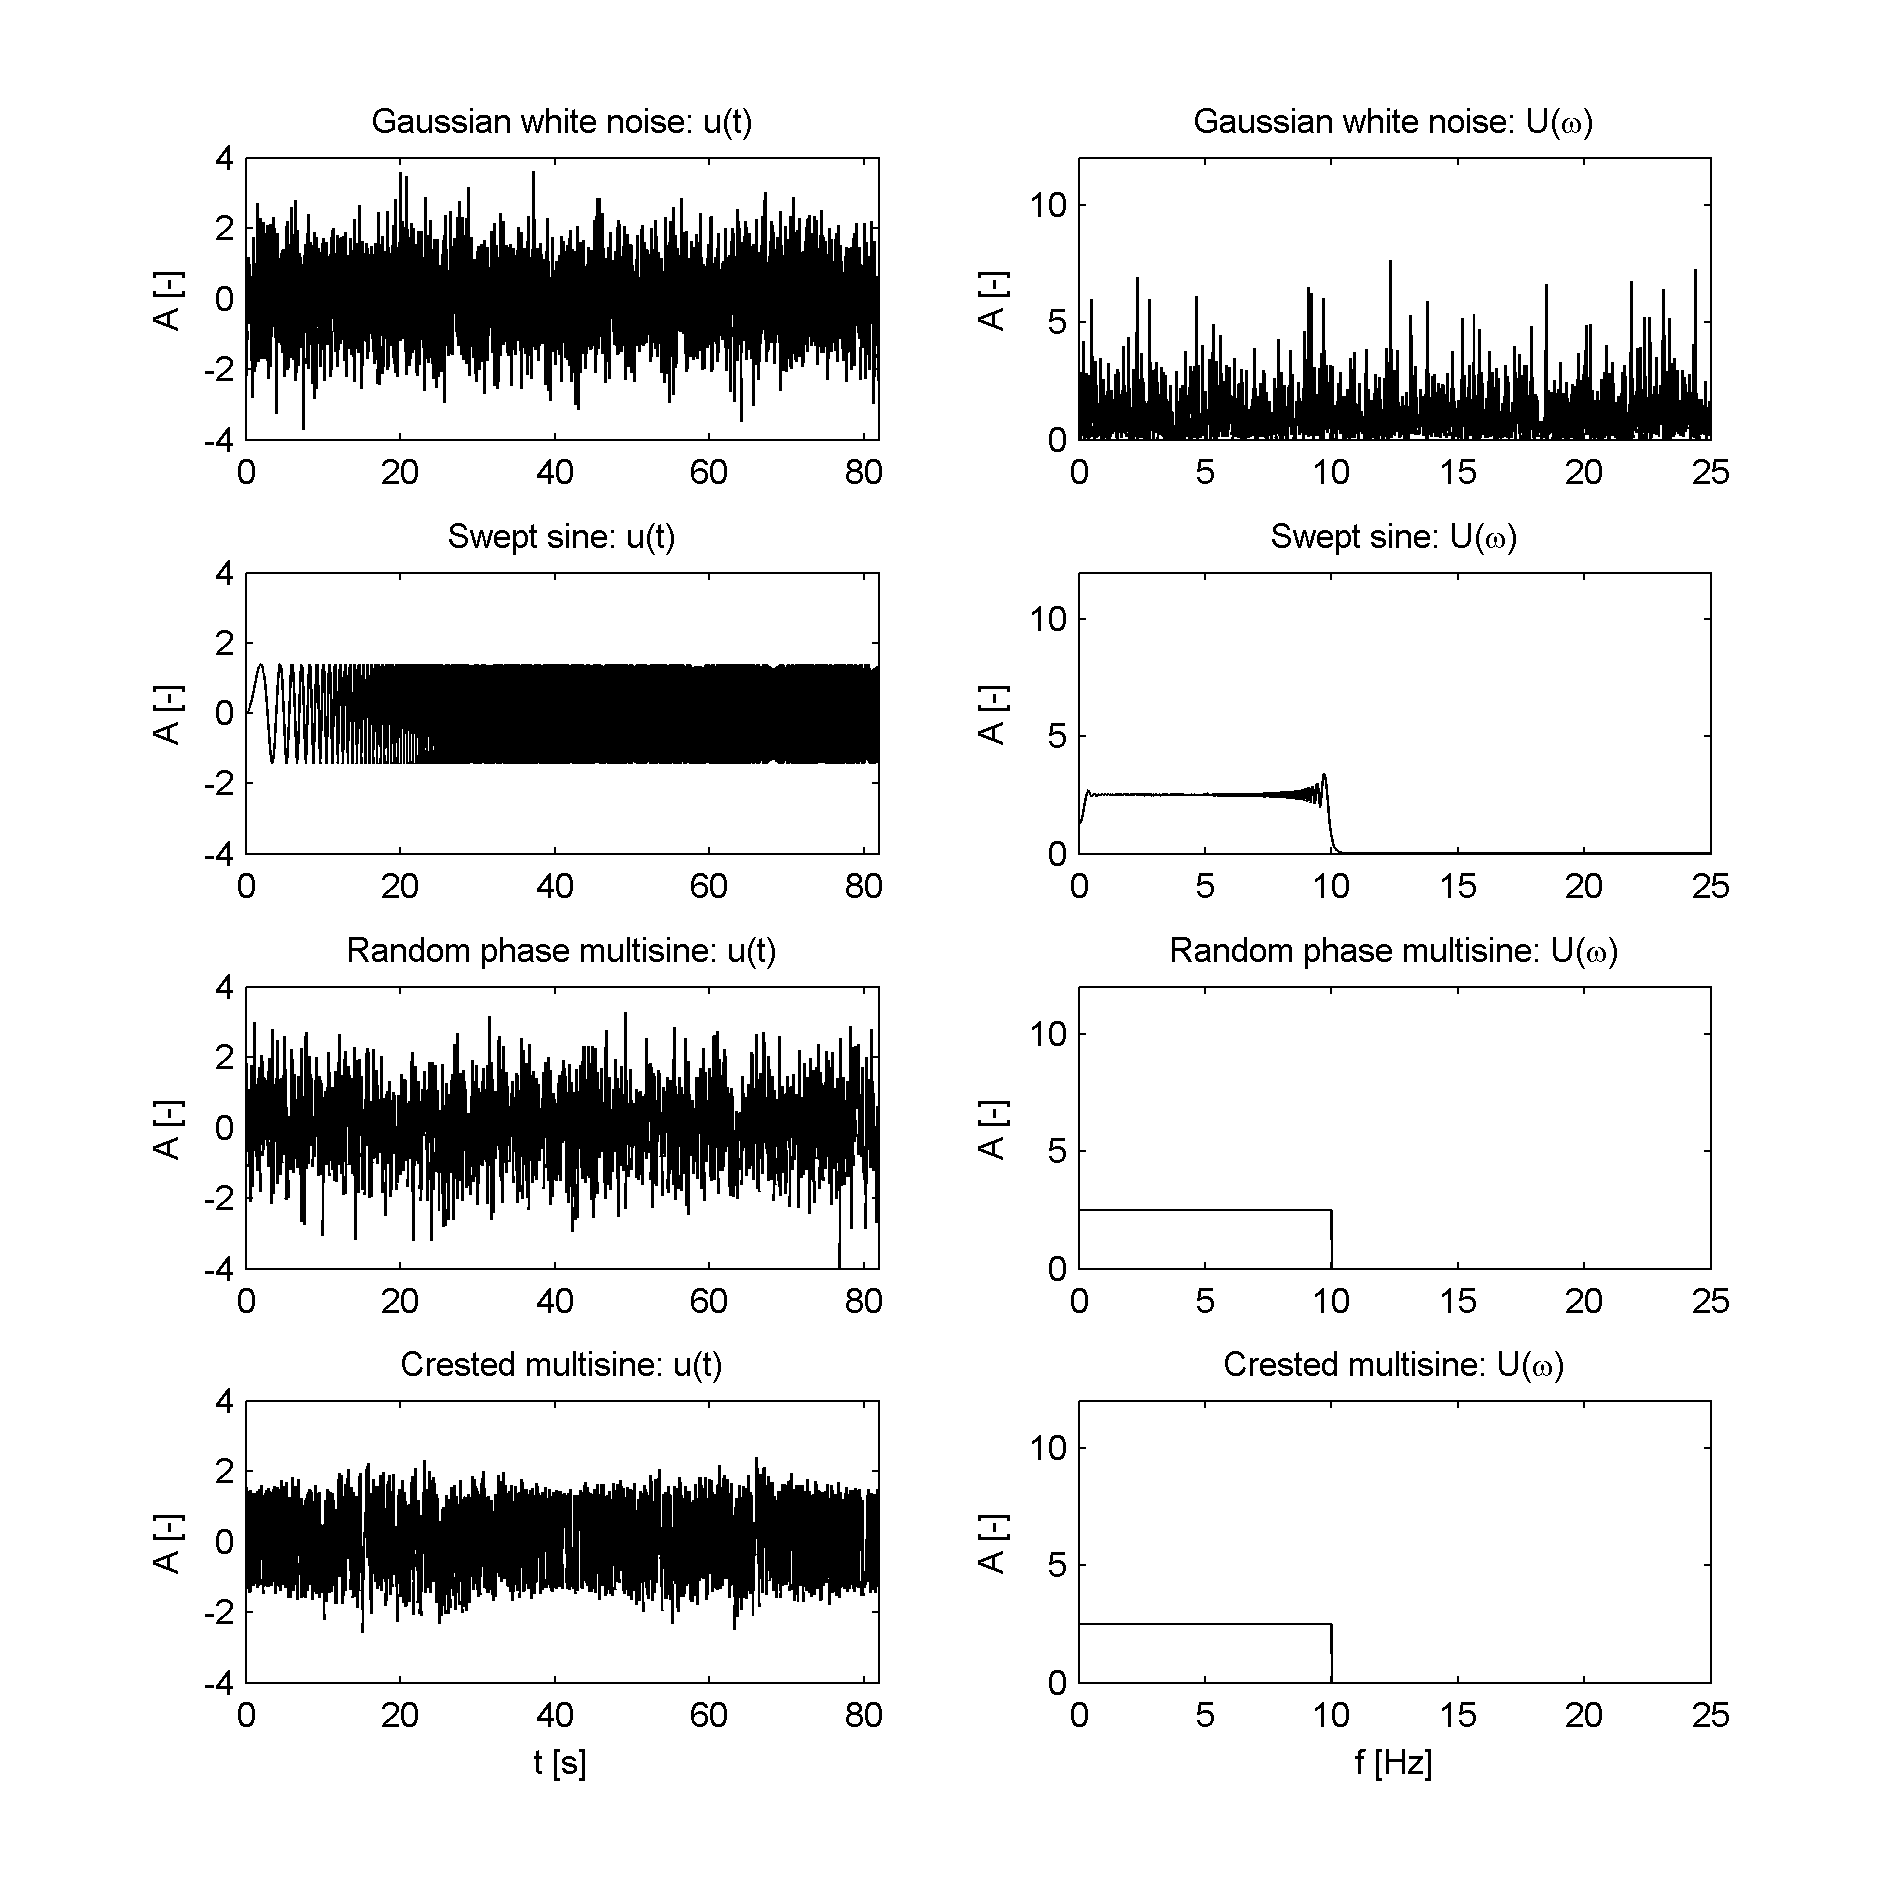
\includegraphics{images/u}
			\label{fig:u}
			\caption{4 different input signals: Gaussian white noise, swept sine, random phase multisine, crested random phase multisine}
		\end{figure}
\begin{table}
		\centering
		\begin{tabular}{lrrrr}
		\toprule
																			& White noise & Swept sine & Multisine & Crested  \\
		\midrule
		Mean ($\mu_u$):					& 0 & 0 & 0 & 0 \\
		Correlation ($R_{uu}$):	& 1 & 1 & 1 & 1 \\
		Spectral density ($S_{uu}):$ 										& 1.0145 &   2.4912  &  2.5000  &  2.5000 \\
		Crest factor ($C$): 						& 3.6129   & 1.4026  &  3.2857   & 2.3943 \\
		Predictable: 								& no & yes & no & no \\
		\bottomrule
		\end{tabular}
		\label{table:u}
		\caption{Comparison of various input signals. Notice that the spectral density is defined as the average spectral density over the desired frequency band.}
\end{table}
\subsection{Results}
The multisine offers the best results, but is predicatable, therefore the crested multisine is advised when identifying  the human controller.